\documentclass[../report.tex]{subfiles}
\begin{document}

\graphicspath{{img/}{../img/}}

\subsection{Business Logic Layer Design}

Our design goals for the Business Logic Layer was to make it:
\begin{enumerate}
\item Transparent
\item Supportable
\item Reliable
\item Testable
\end{enumerate}

In order to gain transparency in our Business Logic Layer we decided to use an Abstract Factory pattern with a regular Factory pattern on top. This makes it possible to gain access to the concrete implementations of the Abstract Factory from the Service Layer while only exposing one concrete class, namely the BusinessLogicEntryFactory. The Service Layer can use the BusinessLogicEntryFactory to get an instance of any of the concrete factories in the Abstract Factory. When it has gotten a concrete factory it cannot see which factory it is using since all the concrete factories have the type IBusinessLogicFactory, nor will it be able to see what concrete product the factory produces.

This makes our Business Logic Layer reasonably transparent. We could have gone for a very transparent design with a Facade pattern for instance. This would mean exposing one concrete class like we do now, but not exposing any interfaces. The way to access the Business Logic Layer would then be by calling a method in the facade class which then delegates the work to other classes in the Business Logic Layer. This would having a method in the facade class for each method in our entire Business Logic Layer making it enormously bloated which works against some of the other goals we are trying to achieve. So we went with the Entry Factory solution because it gives us some of the properties of a Facade Pattern without making a hugely bloated class

The Abstract Factory also helps with the supportability of our Business Logic Layer. The nature of an Abstract Factory makes it very easy to add support for new things by just adding a new factory. In our case the Entry Factory would also have to be updated with a method for creating the new type of factory. Adding completely new functionality is a bit more difficult since the Abstract Factory and/or the Abstract Products interface has to be changed. 

The type of Abstract Factory we have implemented is a very standard kind. We went for this because it is a very reliable kind of Abstract factory compared to a more flexible version which uses parameters in the operations that create objects\footnote{http://www.silversoft.net/docs/dp/hires/pat3afso.htm}. That way of making an Abstract Factory is much less reliable since there is no type security for the products produced by the factories. This can be a big problem for the one who has to use the Abstract Factory.

Another thing that adds to the reliability of our Business Logic Layer is the Entry Factory. Since it is the only concrete class we expose, all interaction with the Business Logic Layer is limited to the methods that our Entry Factory contains. This makes it more difficult to perform unsafe operations.

A lot of reliability also comes from testing so we made sure that our Business Logic Layer is highly testable by interfacing almost everything so it can be unit tested effectively. Apart from interfacing the factories and the products as the Abstract Factory pattern specifies we also interfaced our MediaItemMapper so it could be tested separately. 

Apart from testability the large amount of interfaces also made it possible for us to quickly make a test factory with a stub implementation. This allowed us to deploy something that the SMU students could work with very quickly while simultaneously working on the actual implementation. When the time came to deploy some of the actual implementation we just had to change factories.

\begin{landscape}

\newgeometry{left=1cm,right=-3cm}

\subsection{Class Diagram}

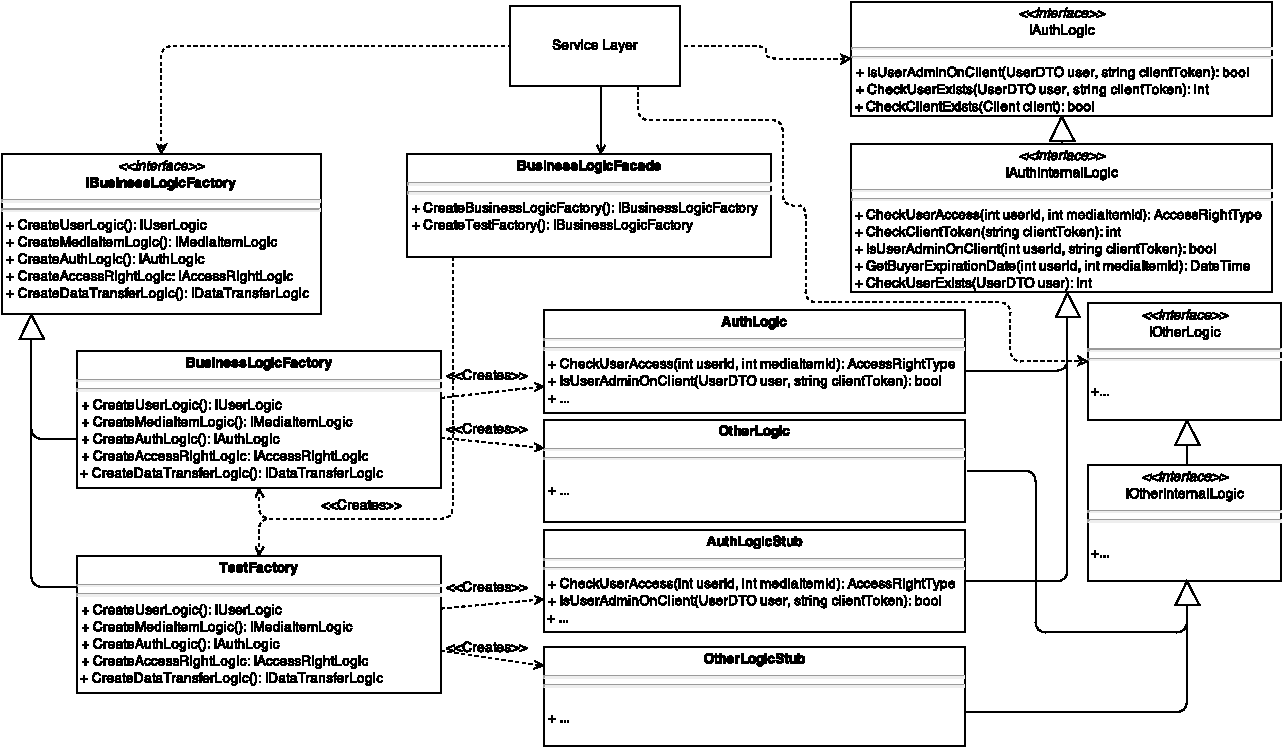
\includegraphics[ scale=1.2]{BusinessLogicLayerDiagram.pdf}

\end{landscape}

The diagram above shows the class structure in the Business Logic Layer. The Entry Factory consists of a single concrete class which in our case is the BusinessLogicEntryFactory class. The BusinessLogicEntryFactory class makes it possible to get hold of the concrete factories without exposing the factories to the Service Layer.

Underneath the Entry Factory lies the Abstract Factory pattern which starts with the Abstract Factory interface which in our case is the IBusinessLogicFactory. This interface specifies a method for creating each of the Abstract Products in this Abstract Factory. The Abstract Products are IAuthLogic, IUserLogic, IMediaItemLogic, IAccessRightLogic and IDataTransferLogic. We then have two concrete implementations of this interface and those are the BusinessLogicFactory and the TestFactory classes. Each of the concrete factories can then produce an instance of a concrete implementation of each Abstract Product. These concrete implementations must implement the Abstract Product interface which contains the methods that are exposed to the Service Layer. But they must also implement an internal interface (ie. IAuthInternalLogic) which specifies methods that are used internally in the Business Logic Layer. These internal interfaces make it possible for the different concrete logic classes to expose methods to one another but not to the Service Layer.

\end{document}